\section{Support Vector Machines}

\subsection{Linear support vector machines}
Figure~\ref{fig:svm-l} shows the results of a single support vector machine with a linear kernel function. As we can see, the results are quite satisfying. The accuracy is high, nevertheless, the results must be nuanced. Indeed, the accuracy doesn't take into account the initial distribution of the classes. This is very important if the initial distribution of a class is not uniform. Let us imagine a data-set where a same class represents a vast majority of the instances -- let's say 90\%. If we imagine a classifier that classifies this class very well and the other classes in a totally not satisfying way, the accuracy would be very high as the main class would weigh a lots in it. This would not be the case with Matthew's correlation coefficient, which takes into account the ratios between the classes. A lower Matthew's correlation coefficient may indicate some classes that are not making a big part of the data and thus weigh not so much on the accuracy, but are still often miscalssified.

\begin{figure}
        \begin{subfigure}[b]{1\textwidth}  
            \centering 
            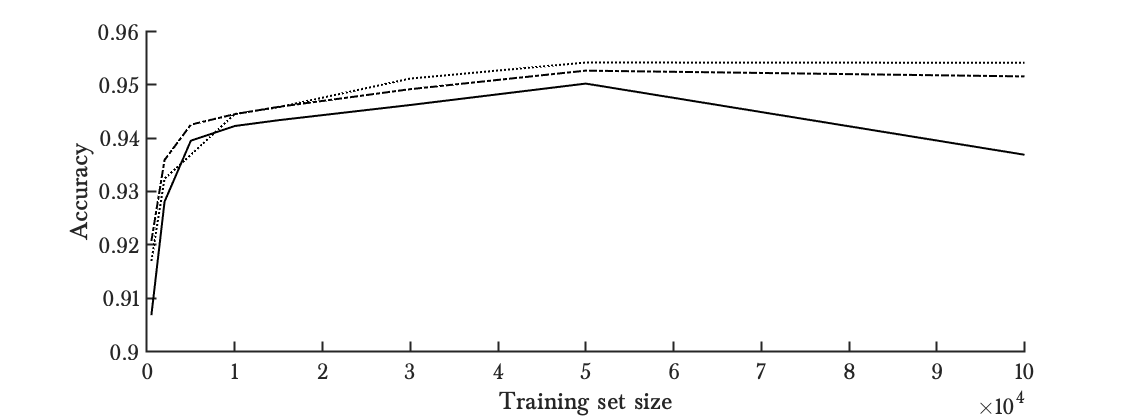
\includegraphics[width=.98\textwidth]{parts/chap-4/img-svm/lin-svm-1.png}
            \caption{Mean Accuracy on the test set.} 
        \end{subfigure}
        \vfill
        \begin{subfigure}[b]{1\textwidth}   
            \centering 
            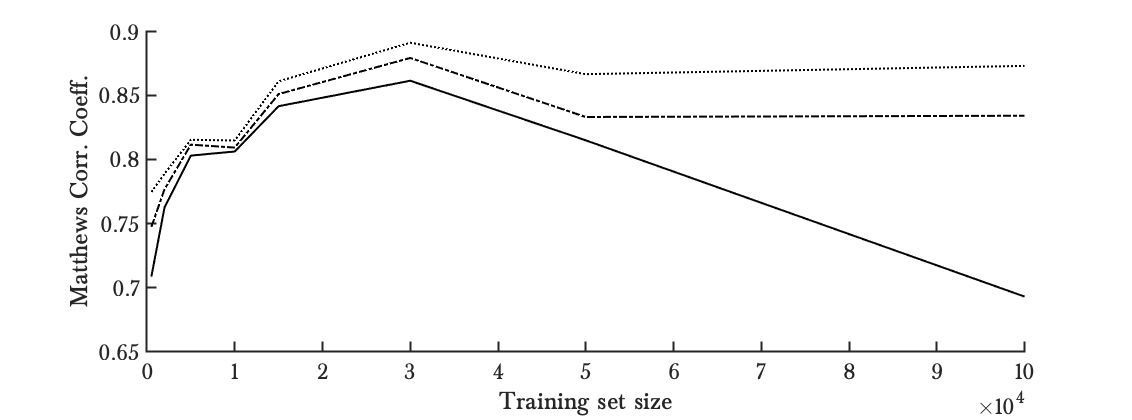
\includegraphics[width=.98\textwidth]{parts/chap-4/img-svm/lin-svm-2.png}
            \caption{Mean Mathews correlation coefficient.} 
        \end{subfigure}
        \vfill
        \begin{subfigure}[b]{1\textwidth}   
            \centering 
            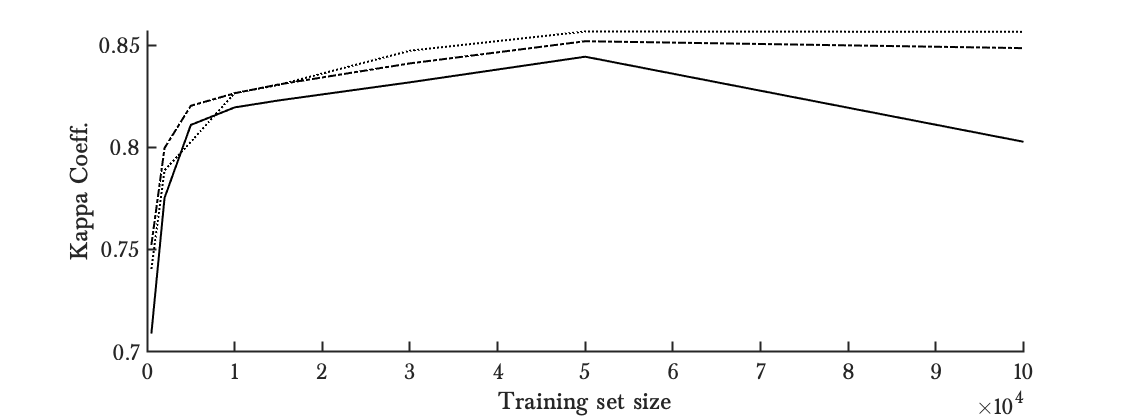
\includegraphics[width=.98\textwidth]{parts/chap-4/img-svm/lin-svm-3.png}
            \caption{Mean Cohen's kappa coefficient.} 
        \end{subfigure}
        \caption{Evaluation of three different models in function of the training set size. The one-against-all (or parallel) model is in dash-dotted line, the tree-bases model (or parallel) are the plain and dotted line. For the plain line, the order of the SVMs is \{Normal, DoS, Prob, R2L, U2R\} and the dotted line is \{Probe, U2R, R2L, DoS, Normal\}. Every result is the mean of 5 different experiments with different training and test set.}
        \label{fig:svm-l}
\end{figure}

Cohen's kappa score indicates something similar. A high value Indeed, We therefore must have a more detailed look at the results (table~\ref{tab:svm-l-1} and \ref{tab:svm-l-2}).

\begin{table}[ht!]
    \centering
    \begin{tabularx}{\textwidth}{lcccccc}
    \hlineI
    Model & Normal & Probe & Dos & R2L & U2R & Total \\ \hlineI
    \textbf{Tree 1} $n=30,000$ & & & & & &\\
    Accuracy [\%] & 76.83 & 93.51 & 92.91 & 92.02 & 80.36 & \\
    MCC & & & & & &  \\
    Kappa & & & & & &  \\
    Obs. Normal  & 1 & 1 & 1 & 1 & 1 & 1\\
    Obs. Probe  & 1 & 1 & 1 & 1 & 1 & 1\\
    Obs. DoS  & 1 & 1 & 1 & 1 & 1 & 1\\
    Obs. R2L  & 1 & 1 & 1 & 1 & 1 & 1\\
    Obs. U2R  & 1 & 1 & 1 & 1 & 1 & 1\\ \hline
    
    \textbf{Tree 2} $n=30,000$ & & & & & &\\
    Accuracy [\%] & 76.83 & 93.51 & 92.91 & 92.02 & 80.36 & \\
    MCC & & & & & & \\
    Kappa & & & & & & \\
    Obs. Normal  & 1 & 1 & 1 & 1 & 1 & 1\\
    Obs. Probe  & 1 & 1 & 1 & 1 & 1 & 1\\
    Obs. DoS  & 1 & 1 & 1 & 1 & 1 & 1\\
    Obs. R2L  & 1 & 1 & 1 & 1 & 1 & 1\\
    Obs. U2R  & 1 & 1 & 1 & 1 & 1 & 1\\ \hline
    
    \textbf{O-A-A} $n=30,000$ & & & & & &\\
    Accuracy [\%] & 76.83 & 93.51 & 92.91 & 92.02 & 80.36 & \\
    MCC & & & & & & \\
    Kappa & & & & & & \\
    Obs. Normal  & 1 & 1 & 1 & 1 & 1 & 1\\
    Obs. Probe  & 1 & 1 & 1 & 1 & 1 & 1\\
    Obs. DoS  & 1 & 1 & 1 & 1 & 1 & 1\\
    Obs. R2L  & 1 & 1 & 1 & 1 & 1 & 1\\
    Obs. U2R  & 1 & 1 & 1 & 1 & 1 & 1\\ \hlineI
    \end{tabularx}
    \caption{Detailed results of the $k$-NN classification algorithm for two different values of the number of neighbours $k$ and for a big and a small training data-set. The accuracy, true positive rate (TP), true negative rate (TN), false positive rate (FP) and false negative rate (FN) are given for each target class.}
    \label{tab:svm-l-1}
\end{table}
    
\begin{table}[ht!]
    \centering
    \begin{tabularx}{\textwidth}{lcccccc}
    \hlineI
    Model & Normal & Probe & Dos & R2L & U2R & Total \\ \hlineI
    \textbf{Tree 1} $n=100,000$ & & & & & &\\
    Accuracy [\%] & 76.83 & 93.51 & 92.91 & 92.02 & 80.36 & \\
    MCC & & & & & & \\
    Kappa & & & & & & \\
    Obs. Normal  & 1 & 1 & 1 & 1 & 1 & 1\\
    Obs. Probe  & 1 & 1 & 1 & 1 & 1 & 1\\
    Obs. DoS  & 1 & 1 & 1 & 1 & 1 & 1\\
    Obs. R2L  & 1 & 1 & 1 & 1 & 1 & 1\\
    Obs. U2R  & 1 & 1 & 1 & 1 & 1 & 1\\ \hline
    
    \textbf{Tree 2} $n=100,000$ & & & & & &\\
    Accuracy [\%] & 76.83 & 93.51 & 92.91 & 92.02 & 80.36 & \\
    MCC & & & & & & \\
    Kappa & & & & & & \\
    Obs. Normal  & 1 & 1 & 1 & 1 & 1 & 1\\
    Obs. Probe  & 1 & 1 & 1 & 1 & 1 & 1\\
    Obs. DoS  & 1 & 1 & 1 & 1 & 1 & 1\\
    Obs. R2L  & 1 & 1 & 1 & 1 & 1 & 1\\
    Obs. U2R  & 1 & 1 & 1 & 1 & 1 & 1\\ \hline
    
    \textbf{O-A-A} $n=100,000$ & & & & & &\\
    Accuracy [\%] & 76.83 & 93.51 & 92.91 & 92.02 & 80.36 & \\
    MCC & & & & & & \\
    Kappa & & & & & & \\
    Obs. Normal  & 1 & 1 & 1 & 1 & 1 & 1\\
    Obs. Probe  & 1 & 1 & 1 & 1 & 1 & 1\\
    Obs. DoS  & 1 & 1 & 1 & 1 & 1 & 1\\
    Obs. R2L  & 1 & 1 & 1 & 1 & 1 & 1\\
    Obs. U2R  & 1 & 1 & 1 & 1 & 1 & 1\\ \hlineI
    \end{tabularx}
    \caption{Detailed results of the $k$-NN classification algorithm for two different values of the number of neighbours $k$ and for a big and a small training data-set. The accuracy, true positive rate (TP), true negative rate (TN), false positive rate (FP) and false negative rate (FN) are given for each target class.}
    \label{tab:svm-l-2}
\end{table}

\begin{wrapfigure}[12]{r}{0.45\textwidth}
\begin{center}
    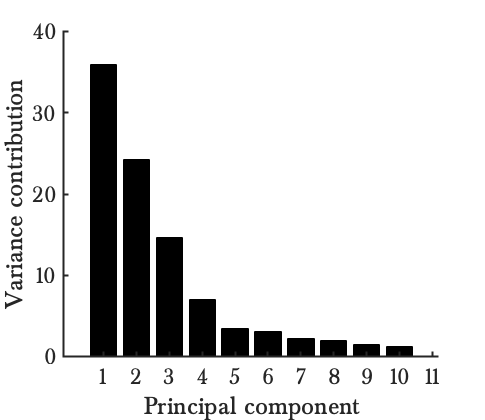
\includegraphics[width=.45\textwidth]{parts/chap-4/img-svm/pca-var.png}
    \caption{Variance participation of the 11 first support vectors.}
    \label{fig:pca-var}
\end{center}
\end{wrapfigure}

\subsubsection{PCA reduction}
Let us now investigate how a principal components decomposition affects the accuracy and allows us to win execution time. The variance contribution of the first principal components is given at figure~\ref{fig:pca-var}.

\begin{figure}
    \centering
    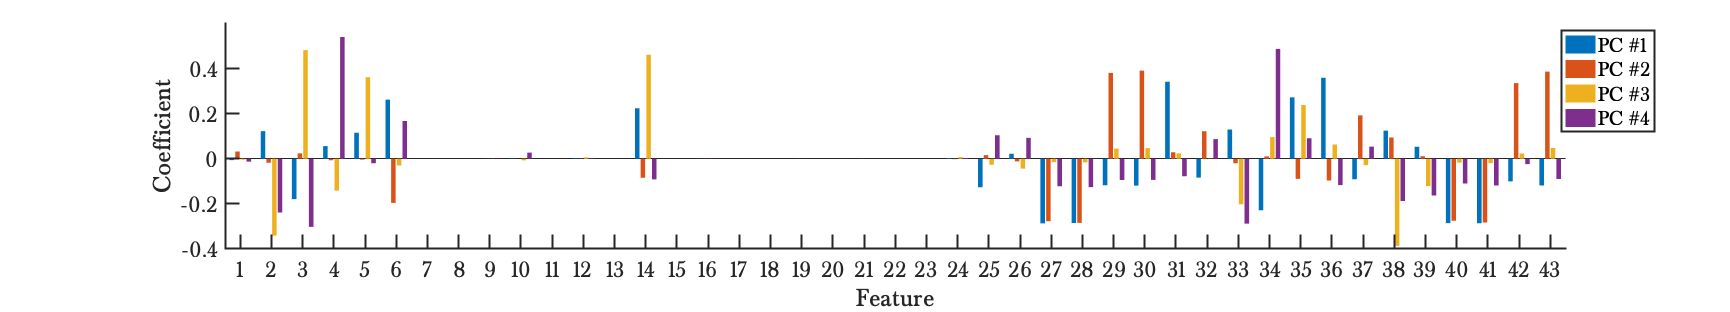
\includegraphics[width=1.\textwidth]{parts/chap-4/img-svm/pca-features.png}
    \caption{Caption}
    \label{fig:pca-features}
\end{figure}

\begin{figure}
        \begin{subfigure}[b]{1\textwidth}  
            \centering 
            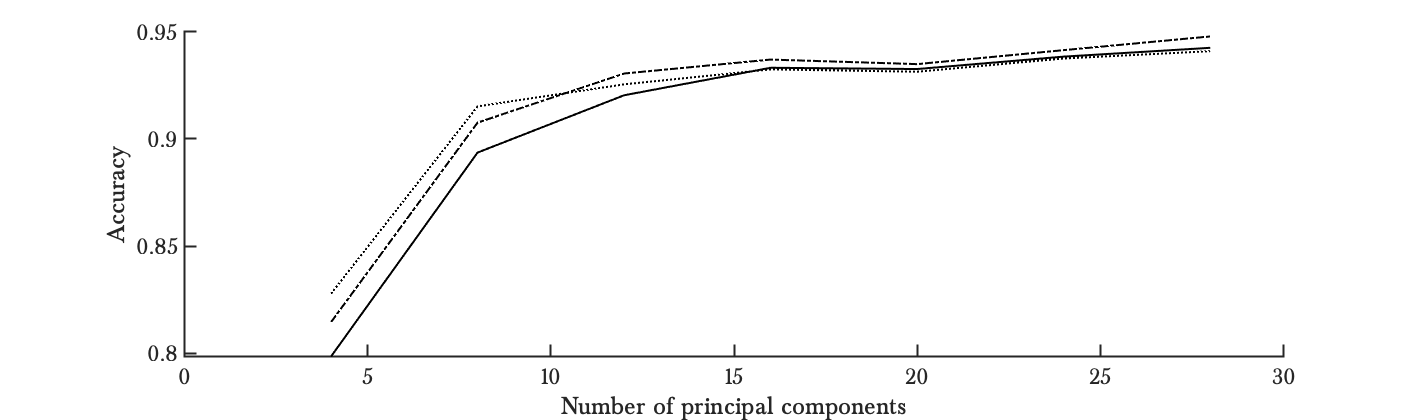
\includegraphics[width=.98\textwidth]{parts/chap-4/img-svm/pca-acc.png}
            \caption{Mean of the accuracy on the test set.} 
        \end{subfigure}
        \vfill
        \begin{subfigure}[b]{1\textwidth}   
            \centering 
            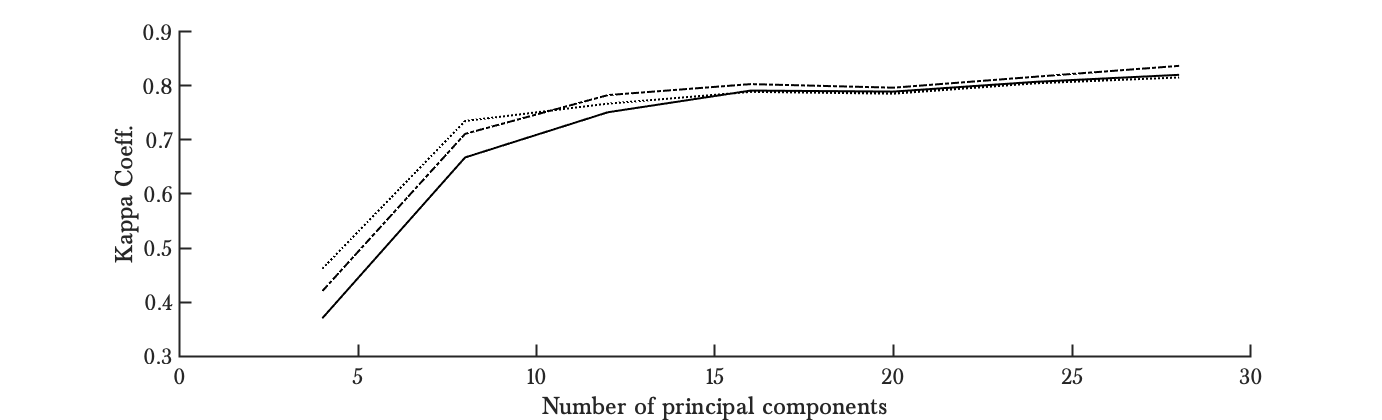
\includegraphics[width=.98\textwidth]{parts/chap-4/img-svm/pca-kappa.png}
            \caption{Mean of Cohen's kappa coefficient.} 
        \end{subfigure}
        \caption{Evaluation of three different models in function of the training set size. The one-against-all (or parallel) model is in dash-dotted line, the tree-bases model (or parallel) are the plain and dotted line. For the plain line, the order of the SVMs is \{Normal, DoS, Prob, R2L, U2R\} and the dotted line is \{Probe, U2R, R2L, DoS, Normal\}. Every result is the mean of 5 different experiments with different training and test set.}
        \label{fig:svm-l}
\end{figure}

An interesting thing with PCA is to think if we could only perform one of the operations (PCA or SVM) and do the other one in clear.
\begin{itemize}
    \item \textbf{Hidden PCA - Clear SVM.} The first idea of doing the PCA tranfsformation in MPC and evaluating the SVM in clear is not very good. It is very naïve to think that PCA destructs the data in such a way that the transformed feature lose much of their information. By transforming using a principal component analysis, we aim at the exact opposite which is to keep as much variance possible, thus as much as information as possible. By looking hereabove at the results of the classifier after the PCA reduction, we notice that the PCA reduction does approach the same classification performance as without. Using clear SVM has also the results that everyone that participates to the evaluation of the transformed data-point can see its classification result. 
    
    The clear SVM evaluation should therefore be limited to the strict minimum parties, i.e. the model owner sending the SVM-model to the query owner which then performs the classification on its own. In this way, his data-point is always hidden, but the model owner reveals a part of his model. However, this model part is unusable in itself as it needs the PCA transformation, which is still hidden.

    The other possibility to keep the whole model (PCA and SVM) hidden is that the query owner sends its query after PCA to the model owner for him to perform the classification. The owner of the model data, once he knows the transformation of the query point, cannot recover it completely. One can notice than computing the inverse of the PCA reduction will lead to some noisy pre-image in the sense that the pre-image is a not a single data-point but a distribution with variance corresponding to the variance list with the PCA transformation. This ressembles to differential privacy, but we will not go further into this direction. To summarize, this will of course reveal the final output (the eventual attack and its type), but somewhat hide the features about the query (e.g. duration or status of the connection). This justifies the preference for the model owner sending the SVM-model to the query owner which then performs the classification on its own. In this scenario, the owner however keeps all its model protected.
    
    Finally, one should add that this whole idea of computing the principal component analysis in MPC and then the SVM in clear is computationally doubtful as the MPC-based PCA-transformation of the query point demands $\mathcal{O}\left(n_{pca}d\right)$ MPC multiplication operations where $d$ is the feature size and $n_{pca}$ the number of principal components kept, here more than 6 for reasonnable performance. Evaluating multi-class support vector machines without PCA and totally hidden has a complexity of $\mathcal{O}(n_{svm}d)$ MPC multiplication operations where $n_{svm}$ is the number of SVMs in the multi-class model, here 4 or 5 depending on which model structure is used. Once the PCA transformation is complete, you still have to add the designation of a winner between the different binary SVMs output which takes $\mathcal{O}(n_{svm})$ MPC comparison operations which are known to be more expensive than multiplications. Figure~\ref{} compares the difference between those two method and concludes that this trade-off isn't very conclusive and one should prefer computing the whole SVM in MPC without any PCA reduction. Indeed the the fact that $n_{pca} > n_{svm}$ isn't compensated by the hidden designation of a winner.
    
    \item \textbf{Clear PCA - Hidden SVM.}
    This alternative has the same property as before, the model is still partially hidden. Furthermore, the hidden evaluation of the SVM guarantees the privacy of the final classification output. Conversely as before, the question of whom evaluates the PCA decomposition has only one possibility, the query owner as the opposite would reveal the initial feature vector to someone else and loose all the privacy of the queried point.
    
    The first question if we reveal the PCA components is what information is revealed. Well, not much as this is the result of the sole diagonalization of the correlation matrix of the model owner's initial data-points. The correlation matrix instrisically reveals the linear relations between different features. This would harshly reveal anything about the original data-points as this relation is computed amongst ideally several thousands of points from all classes alltogether. Furthermore, this correlation matrix is diagonalized and the sole first components are kept, revealing in a certain sense the sole important relations. With the hypothesis that each class has different subjacent relations and thus different principal components \noteH{maybe test this hypothesis ?}, an attacker could --- but this is going quite far --- deduce which classes were present in the model owner original data-set and thus deduce to which attack he is subject to, or at least detected. However, the exact nature of the original individual data-points remains secret and so does the queried data-point as it never leaves its owner in clear form.
    
    The advantage of this method is that performing an hidden SVM with pre-computed PCA reduction reduces the complexity from $\mathcal{O}(n_{svm}d)$ to $\mathcal{O}(n_{svm}n_{pca})$ and in the practice of a factor between 2 and 4. However, the designation of the winning SVM remains $\mathcal{O}(n_{svm})$.
    
    \item \textbf{No PCA - Clear SVM.} In this case, the query owner recieves the whole model from the model owner. Of course, not much here is still hidden. In fact, all the model is clear an can be used by anybody who recieves it and there is no need at all for MPC techniques. However linear SVM have the big advantage against the other ones, using kernel trick, that it doesn't need the dual to be computed. This means that instead of sending the $\alpha_i$ with their corresponding support vectors $x_i$ and targets $l_i$ (which will be of course a huge breach of privacy-friendliness), one can just send the weights vector $w$ (and the bias $b$), which reveals much less information about the model. The exact relation between the weights and the support vectors is 
    \begin{equation}
        w = \sum_{\forall i}\alpha_i l_i x_i
    \end{equation}
    The bias stays the same. The computation of the wieghts is of course a very big compression of the support vectors and destroys the information they contain. In this sense, a totally clear model could be an option, depending on the choices of the model owner. Considering the execution speed, this has no competitor among the model we test as avoiding the use of MPC leads to drastic speed evaluations. A drawback however, that has less to do with privacy-friendliness but is still relevant is the loss of control the owner of the model gets with this method. Indeed, the big advantage of using MPC on a significant part of the model is that the other celar parts of the model are unusable without the MPC-part, whose parameters are never revealed. In this sense, the owner of the data still has a full control as he is the sole who can ultimately decide whether or not his model can be used. Once all is in clear, this property disappears and there is no more secure lock against the proliferation of the models use without its consent. This can be relevant for commercial uses for example\footnote{Besides, this raises an interesting question on how to secure software against illegal proliferation and use. Instead of using license keys, why just not performing a very small, but essential task in MPC without which the program could possibly work (in an information-theoretic scheme). In this sense, the owner is sure that only identified users --- which he can control at each instant --- are allowed to use the program. This of course would need to rest on a permanent internet connection (which is nowadays less a problem, more and more smartphone apps are requiring a permanent internet connection) and avoiding the MPC task being cracked and substituted by local version. This is a totally out of the scope of my thesis, but I believe the question to be interesting. Of course, this idea could also be used without MPC and just data snet in ean encrypted form, but this would not be privacy-friendly for the user. Another question would also be, who be the third party to avoid a malicious majority, the first party being the user and the second the company. The third party would be a party that has no interest in working with the user and thus cracking the program nor with the firm issuing the program revealing the user's data. This could be repalced by homomorphic encryption to avoid the use a of third party but is computationally more \noteH{?} costly.}.
\end{itemize}

\subsubsection{$\chi^2$-reduction}
Where the PCA decomposition is the same for all binary SVM, the $\chi^2$ feature selection allows us to select the most relevant features for each SVM. This allows us for a more specifically pre-processed classifiers. Here, the big advantage is a reduction of complexity from $\mathcal{O}(n_{svm}d)$ to $\mathcal{O}(n_{svm}n_{\chi^2})$.

\subsection{Non-linear support vector machines}

Figure~\ref{} shows the results of a radial based function support vector machine on the NSL-KDD data-set. The box constraints $C$ and the kernel function parameter $\sigma^2$ are optimized at each specific training through a 10-fold cross-validation.

It seems that there is a \noteH{plafond de verre} that a higher number of training elements cannot break. One may also be surspised by the relatively low results achieved by the classification. However, a very interesting result appears when we try not to use the test set given in the data-set. Figure~\ref{} shows the same results, but based on a division of the original training set into a new training and test set. To obtain a fair comparison, both testing set have the same size and the same proportions of the different classes inside it. These results are much higher and suggest that the original testing data-set is statistically much different than the training set. This makes the classification problem much more difficult as it must predict data for which to doesn't have learned anything similar. This asks for more generalization. However, one may have a look to the specific results of each binary classifier that are here much better (table~\ref{}).

The number of support vector machines has a very high influence on the speed of the evaluation through MPC. A very interesting observation is that the tree-based classifier do not perform worse that the one-against-all model. Indeed, the order of the tree-based is very important as it can make the tree-based model perform better or worse than one-against-all models. In this sense, the best tree-based structure does perform better and has a faster evaluation through MPC as it comprises one SVM less.
\noteH{more details on comparison one-against-all and tree based models}.

Figure~\ref{} shows how much time each of this classifiers take to evaluate a single test point. 

As we said before, $C$ is optimized through validation. However, this directly controls the number of support vectors. However, the complexity of the evaluation of the support vector machine is linearly dependent on the number of support vectors. Figure~\ref{} shows the total number of support vectors for the one-against-all model and the best sequential classifier. One can see that these are closely related to the speed of the evaluation of the support vector machine through MPC. To improve the speed of the evaluation, one must thus reduce the number of support vectors. This can be controlled by the box constraint $C$ which --- as a reminder --- represents the trade-off between the objective of a support vector machine and the influence of the slack variables --- we could the corresponding data-points the "difficult" ones. In this sense, a high value of $C$ will just make the boundary absolutely fit to every variable and tolerate no wrongly classified data-point to the model. In other words, the difficult data-points will have a much higher influence. This is even more clear in the dual as the box constraint $C$ directly represents an upper bound on the $\alpha_i$. A high value of $C$ leads to less regularization and the model to fit to these specific difficult points, which increases the risk of overfitting. Let's investigate how far we can increase the box constraint $C$ without suffering from overfitting. By this mean, we can reduce the MPC evaluation without having too much impact on the accuracy.